% Paper 2 — grounded lenstronomy code generation with sandboxed validation.
% ML4PS @ NeurIPS workshop, 4-page limit. Style: official neurips_2025.sty
% (vendored; TODO swap for the ML4PS 2026 template when released).
\documentclass{article}
\usepackage[final]{neurips_2025}

\usepackage[utf8]{inputenc}
\usepackage[T1]{fontenc}
\usepackage{hyperref}
\usepackage{url}
\usepackage{booktabs}
\usepackage{amsfonts}
\usepackage{microtype}
\usepackage{graphicx}
\usepackage{xcolor}
\usepackage{tikz}
\usetikzlibrary{arrows.meta, positioning}

\makeatletter
\renewcommand{\@noticestring}{%
  Machine Learning and the Physical Sciences Workshop, NeurIPS 2026.\ % TODO: confirm exact ML4PS 2026 footer wording
}
\makeatother

\newcommand{\todo}[1]{\textcolor{red}{[TODO: #1]}}

\title{Version-Grounded LLM Code Generation for Strong-Lensing Simulation:
Sandboxed Execution and Validation for DeepLenseSim}
% TODO: working title — refine with co-authors.

% TODO: author order / lead for this paper unconfirmed (Michael's and Luca's
% involvement TBD) — placeholder order below.
\author{%
  Aatmaj Amol Salunke\\
  Northeastern University\\
  \texttt{\todo{email}}\\
  \And
  Pranath Reddy\\
  University of Florida\\
  \texttt{\todo{email}}\\
  \And
  Michael W.\ Toomey\\
  Massachusetts Institute of Technology\\
  \texttt{\todo{email}}\\
  \And
  Sergei Gleyzer\\
  University of Alabama\\
  \texttt{\todo{email}}\\
}

\begin{document}

\maketitle

\begin{abstract}
\todo{150--200 words. (1) Problem: producing new strong-lensing simulation
variants requires hand-writing lenstronomy scripts against a version-fragile API;
naive LLM codegen emits plausible-but-broken calls (version blending). (2) System:
natural-language spec $\to$ LLM codegen grounded by an introspection-verified,
version-pinned API cheat-sheet $\to$ isolated Docker execution (era-matched
dependency pins) $\to$ structural validation with error-feedback retries.
(3) Results: grounding flips the same model from 0/3 failures to first-attempt
success; 9/9 prompt suite pass rate with gpt-5.2; verified container isolation;
the same stack generated the 9k-image training corpus. (4) Honesty: small
evaluation, structural (not physical) validation, pyHalo grounding open.}
\end{abstract}

\section{Introduction}
\todo{2--3 paragraphs. DeepLense simulation workflow today (hand-written
DeepLenseSim scripts per model class \citep{alexander2020deep,toomey2022deep});
LLM code generation promise vs.\ API-version fragility (lenstronomy 1.9.2 vs
1.14+: \texttt{numPix}$\to$\texttt{num\_pix}, PSF \texttt{sigma} vs
\texttt{fwhm}); contribution: (a) version-grounding via introspected cheat-sheet,
(b) hardened sandbox with era-matched pins, (c) validation/retry loop, (d) honest
evaluation. One sentence situating this within the broader DLens agent framework
(the AI-scientist loop is a separate paper).}

\section{System}
\label{sec:system}
\todo{Describe Figure~\ref{fig:flow}: SimSpec (NL) $\to$ grounded codegen agent
(cheat-sheet: exact 1.9.2 signatures, regenerated by introspection inside the
image) $\to$ GeneratedProgram $\to$ DockerSandbox (non-root uid 10001, no network,
2\,GB/1-CPU cgroup caps, timeout, mounted job dir, DLENS\_OUTPUT convention)
$\to$ structural validation (finite non-trivial 2-D image) $\to$ error-feedback
retry ($\le$3 attempts) $\to$ CodegenResult with reasoning. Era-matched pins
(numpy$<$2, scipy$<$1.14, astropy$<$6, pyHalo@2022) as part of the grounding
story.}

\begin{figure}[t]
  \centering
  % TODO: replace stub with the real system figure before submission.
  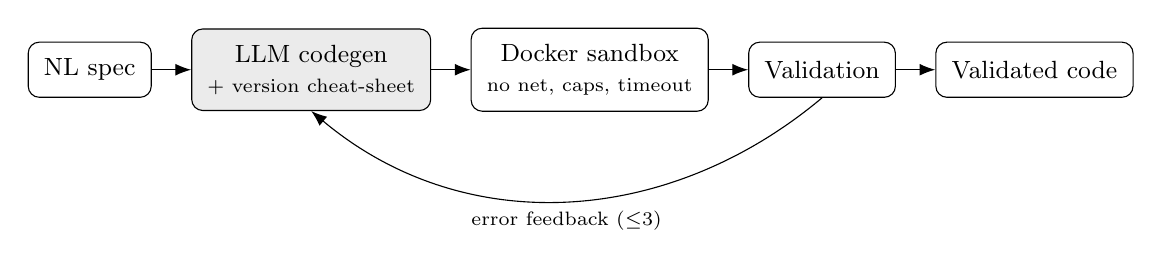
\begin{tikzpicture}[
      node distance=3mm and 5mm,
      stage/.style={draw, rounded corners, minimum height=7mm, inner sep=2mm,
                    font=\small, align=center},
      arr/.style={-{Latex[length=2mm]}}
    ]
    \node[stage] (nl) {NL spec};
    \node[stage, right=of nl, fill=black!8] (gen) {LLM codegen\\{\scriptsize + version cheat-sheet}};
    \node[stage, right=of gen] (sbx) {Docker sandbox\\{\scriptsize no net, caps, timeout}};
    \node[stage, right=of sbx] (val) {Validation};
    \node[stage, right=of val] (out) {Validated code};
    \draw[arr] (nl) -- (gen);
    \draw[arr] (gen) -- (sbx);
    \draw[arr] (sbx) -- (val);
    \draw[arr] (val) -- (out);
    \draw[arr] (val.south) to[out=-140, in=-40] node[below, font=\scriptsize]
      {error feedback ($\le$3)} (gen.south);
  \end{tikzpicture}
  \caption{\todo{Final caption.} Natural language to validated, executable
  lenstronomy simulation code.}
  \label{fig:flow}
\end{figure}

\section{Evaluation}
\label{sec:eval}
\todo{Setup: 9 synthetic prompts derived from DeepLenseSim Models I--III $\times$
\{no\_sub, cdm, axion\}; max 3 attempts; identical settings per model; real API
calls + real container execution. Grounding before/after: same model (gpt-5.2),
same request — 0/3 attempts without the cheat-sheet vs.\ first-attempt pass with
it. Isolation verification (Table~\ref{tab:isolation}). Scale data point: the
same stack generated the 9{,}000-image training corpus used by the companion
pipeline work.}

\begin{table}[t]
  \caption{Model comparison on the 9-prompt suite (real generation + sandboxed
  execution; max 3 attempts). gpt-5.6-luna requires the OpenAI Responses API for
  structured output; its one failure is a pyHalo import outside the cheat-sheet's
  coverage.}
  \label{tab:models}
  \centering
  \small
  \begin{tabular}{lcc}
    \toprule
    Metric & gpt-5.2 & gpt-5.6-luna \\
    \midrule
    Final pass (validated image) & \textbf{9/9} & 8/9 \\
    First-attempt pass & 2/9 & 3/9 \\
    Mean attempts & 1.78 & 1.78 \\
    Structured output ok / code parses & 16/16 / 16/16 & 16/16 / 16/16 \\
    Mean generation latency (s) & 13.7 & \textbf{9.4} \\
    Mean wall time per prompt (s) & 26.0 & \textbf{18.1} \\
    \bottomrule
  \end{tabular}
\end{table}

\begin{table}[t]
  \caption{Sandbox isolation, verified from inside the container via the
  production execution path.}
  \label{tab:isolation}
  \centering
  \small
  \begin{tabular}{ll}
    \toprule
    Property & Observed \\
    \midrule
    Guest OS & Linux (linuxkit) vs.\ Darwin host \\
    User & non-root \texttt{sandbox}, uid 10001 \\
    Network & blocked (\texttt{OSError} on connect; \texttt{--network=none}) \\
    Memory / CPU caps & cgroup \texttt{memory.max} = 2\,GiB; \texttt{cpu.max} = 1 CPU \\
    Scientific stack & lenstronomy 1.9.2 executed in-container \\
    \bottomrule
  \end{tabular}
\end{table}

\section{Results and Discussion}
\label{sec:results}
\todo{Walk Table~\ref{tab:models}; the grounding before/after; luna's
pyHalo-import failure as evidence that grounding coverage, not model capability,
is the binding constraint (footnote: the import is valid for 2022-era pyHalo —
version blending, not pure hallucination); limitations from the fact sheet
(structural-not-physical validation; small prompt suite; no scientist-authored
ground-truth prompts yet).}

\section{Conclusion}
\todo{3--4 sentences: version-grounding + sandboxed validation makes LLM codegen
for a version-fragile scientific stack reliable enough to hand validated scripts
to simulation leads; next: pyHalo grounding, physics-aware validation, and a
scientist-in-the-loop evaluation with ground-truth prompts.}

\begin{ack}
\todo{Match last year's ML4PS/DeepLense acknowledgement wording.} This work was
supported by Google Summer of Code 2026 with the Machine Learning for Science
(ML4SCI) organization.
\end{ack}

\bibliographystyle{plainnat}
\bibliography{references}

\end{document}
